\section{Theoretische Grundlagen}

Eine Wärmepumpe ist eine Vorrichtung, die in der Lage ist einen Wärmefluss von einem kälteren in ein
wärmeres thermisches Reservoir herzustellen. Dies geschieht entgegen dem normalerweise vorliegendem Prozess,
das die Wärme von einem wärmeren in ein 
kälteres Reservoir fließt.\\
Damit die Wärmepumpe diese Richtung umkehrt muss in ihr,
nach dem zweiten Hauptsatz der Thermodynamik, noch zusätzliche
mechanische Arbeit verrichtet werden.\\
Die vom wärmeren Reservoir aufgenommene Wärmemenge $Q_1$ ist also gleich der
Summe des aus dem vom kälteren Reservoir entnommenen Wärmemenge $Q_2$ und der verrichteten Arbeit $A$:
\begin{equation}
  Q_1 = Q_2 + A  
  \label{eqn:transp}
\end{equation}

\subsection{Güteziffer}

Das Verhältnis zwischen der transportierten Wärmemenge und der 
aufgewendeten Arbeit $v=\frac{Q_1}{A}$ nennt man Güteziffer.\\
Die Güteziffer ist ein Maß für die Effektivität einer Wärmepumpe.\\
Aus dem zweiten Hauptsatz der Thermodynamik lässt sich zusätzlich auch noch herleiten,
dass die Summe der reduzierten Wärmemenge null sein muss.
\begin{equation}
    \frac{Q_1}{t_1}-\frac{Q_2}{T_2}=0
\end{equation}
Durch einsetzen der letzten beiden Formeln und \refeq{eqn:transp} ineinander
ergibt sich eine Aussage für die ideale und damit maximal mögliche Güteziffer:
\begin{equation}
    v_\text{ideal}= \frac{T_1}{T_1-T_2}
    \label{eqn:videal}
\end{equation}
Hier zeigt sich, dass die Effektivität einer Wärmepumpe
umso größer ist, desto kleiner die Temperaturdifferenz der Reservoire ist. \\
Die reale Güteziffer $v_\text{real}$ muss offensichtlicherwiese
kleiner als $v_\text{ideal}$ sein, da nicht alle Arbeit direkt für den zuvor 
beschriebenen Prozess genutzt wird, wodurch insgesamt mehr Arbeit nötig wird.\\
$v_\text{real}$ berechnet sich mit einem über die Differenzenquotienten
einer, über ein Zeitintervall gewonnenen, Wärmemenge und Temperatur.
\begin{equation}
    \frac{\increment Q_1}{\increment t} = \left(m_1 c_w + m_k c_k \right)\frac{\increment T_1}{\increment t}
    \label{eqn:delQ}
\end{equation}
Mit Hilfe der über das Zeitintervall gemittelten Leistungsaufnahme $\symup{N}$
lässt sich dann $v_\text{real}$ bestimmen.
\begin{equation}
    v_\text{real}= \frac{\increment{Q_1}}{\increment t \cdot \symup{N} }
    \label{eqn:vreal1}
\end{equation}\\
Für unsere Rechnungen verwenden wir aber keinen Differenzenquotienten sonderen rechnen mit dem Differential
einer auf die Messwerte gefiteten Funktion.

\subsection{Massendurchsatz}

Der Massendurchsatz ist der Durchsatz des Transportmediums, in diesem Fall
Dichloridfluormethan $\ce{Cl2F2C}$, von einem Abschnitt des Kreislaufs in einen anderen.\\
Da die Wärmeentnahme aus dem kälteren Reservoir durch Verdampfung des Medium geschieht, 
lässt sich mit Hilfe der Verdampfungswärme des Mediums und dem Differenzenquotienten 
der entnommenen Wärmemenge des Reservoirs, der Durchsatz bestimmen.
Dies geschieht über eine zu \refeq{eqn:vreal1} ähnliche Formel, nur mit korrespondierenden
Werten für $T_2$.
\begin{equation}
    \frac{\increment Q_2}{\increment t} = L\cdot \frac{\increment m}{\increment t}
    = \left(m_2 c_w + m_k c_k \right)\frac{\increment T_2}{\increment t}
\end{equation}

\subsection{Die mechanische Kompressorleistung} \label{kompressor}
\begin{align*}
    \intertext{Die Kompressorleistung ergibt sich als die Kompressionsarbeit pro Zeit, also als:}
    N_\text{mech}&=\frac{\increment A_m}{\increment t}
    \intertext{Des Weiteren ist die Kompressionsarbeit die Arbeit, welche verrichtet wird, wenn ein Stoff eines Volumens zu einem anderen Volumen komprimiert wird.}
    A_m&= - \int_{V_a}^{V_b} p \, \symup{d}V
    \intertext{Für die Berechnung der Kompressorleistung  $N_\text{mech}$ darf eine adiabatische Kompression angenommen werden, 
    weswegen die Poissonsche Gelichung genutzt werden kann.}
    p_a V_a^{\kappa} &= p_a V_a^{\kappa} =p V^{\kappa}
    \intertext{Wobei $\kappa$ das Verhältinis der Molwärmen $C_p$ und $C_v$ ist.}
    \intertext{So ergibt sich dann zur Berechnung der Leistung die Formel:}
    N_\text{mech} &= \frac{q}{\kappa-1}\left( p_b \sqrt{\kappa}{\frac{p_a}{p_b}}-p_a \right) \frac{1}{\rho} \frac{\increment m}{\increment t}
\end{align*}
\newpage


\subsection{Arbeitsweise einer Wärmepumpe}

\footnotetext[1]{TU Dortmund. D206 Die Wärmepumpe/Anleitung Wärmepumpe.pdf (2020)}

\begin{figure}
    \centering
    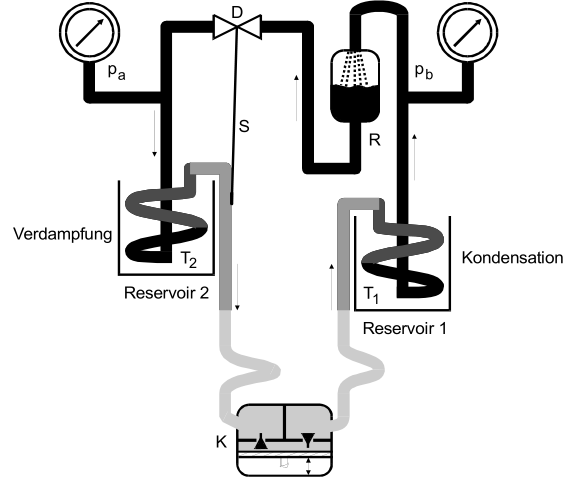
\includegraphics[width=0.7\textwidth]{images/Versuchsaufbau.png}
    \caption{Schematischer Aufbau einer Wärmepumpe \protect \footnotemark[1] ($p_b> p_a; T_1>T_1$).}
    \label{img:pump1}
\end{figure}

Eine Wärmepumpe ist, wie schon erwähnt, eine Vorrichtung um Wärmeenergie aus einem kalten 
Reserovoir, unter Zuführung mechanischer Arbeit, in ein wärmerses Reservoir zu überführen.\\
In \ref{img:pump1} sieht man den schematischen Aufbau einer solchen Pumpe.
Das ganze System ist mit einem Gas gefüllt, welches bei niedrigem Druck unter Wärmezufuhr verdampft
und bei höherem Druck unter Wärmeabgabe kondensiert.
Wenn man ein Gas wählt, das bei $p_b$ und $T_1$ kondensiert und bei $p_a$ und $T_2$ verdampft,
lässt es sich für eine dazu passende Wärmepumpe nutzen.\\
Das Gas wird im Kompressor K adiabatisch verdichtet, also ohne Wärmeverluste an die Umgebung. 
Dabei erhitzt es sich, bleibt aber weiterhin gasförmig. 
Anschließend, beim durchströmen des Reservoirs 1, kann es seine leicht erhöhte thermische Energie
im Reservoir abgeben, wodurch es wieder kondensiert.
In disem vorgang steigen $p_b$ und $T_1$.\\
Als nächstes durchströmt das Transportmedium den Reiniger R, wo es von Gasresten bereinigt wird, 
welche die Vörgange in der Pumpe behindern würden.\\
Nun gelangt das Medium an das Drosselventil D, wo es sich beim Eintritt in $p_a$ entspannt und 
wieder gasförmig wird. Dabei kühlt es sich sehr stark ab.\\
Beim durchlaufen des zweiten Reservoirs, welches wärmer als das Gas ist, gleichen sich Gas- und Reservoir-temperatur aneinander an.\\
Dabei entzieht das Gas dem Reservoir thermische Energie, wodurch sich das Reservoir abkühlt.\\
Schlußendlich durchströmt das Gas wieder den Kompressor und der Kreislauf beginnt von vorne.\\
Die Wärmepumpe entzieht also mit Hilfe des Phasenübergangs des Gases dem zweiten Reservoir Energie, welche dann 
genutzt wird um das erste zu erwärmen.




